\documentclass[25pt, a0paper, landscape]{tikzposter}
\tikzposterlatexaffectionproofoff
\usepackage[utf8]{inputenc}
\usepackage{authblk}
\makeatletter
\renewcommand\maketitle{\AB@maketitle} % revert \maketitle to its old definition
\renewcommand\AB@affilsepx{\quad\protect\Affilfont} % put affiliations into one line
\makeatother
\renewcommand\Affilfont{\Large} % set font for affiliations
\usepackage{amsmath, amsfonts, amssymb}
\usepackage{tikz}
\usepackage{pgfplots}
% align columns of tikzposter; needs two compilations
\usepackage[colalign]{column_aligned}
\usepackage{graphicx}
\graphicspath{{/Users/yuminsun/dl4cvproject/doc/poster/assets/}}

% tikzposter meta settings
\usetheme{Default}
\usetitlestyle{Default}
\useblockstyle{Default}


%%%%%%%%%%% redefine title matter to include one logo on each side of the title; adjust with \LogoSep
\makeatletter
\newcommand\insertlogoi[2][]{\def\@insertlogoi{\includegraphics[#1]{#2}}}
\newcommand\insertlogoii[2][]{\def\@insertlogoii{\includegraphics[#1]{#2}}}
\newlength\LogoSep
\setlength\LogoSep{-70pt}

\renewcommand\maketitle[1][]{  % #1 keys
    \normalsize
    \setkeys{title}{#1}
    % Title dummy to get title height
    \node[inner sep=\TP@titleinnersep, line width=\TP@titlelinewidth, anchor=north, minimum width=\TP@visibletextwidth-2\TP@titleinnersep]
    (TP@title) at ($(0, 0.5\textheight-\TP@titletotopverticalspace)$) {\parbox{\TP@titlewidth-2\TP@titleinnersep}{\TP@maketitle}};
    \draw let \p1 = ($(TP@title.north)-(TP@title.south)$) in node {
        \setlength{\TP@titleheight}{\y1}
        \setlength{\titleheight}{\y1}
        \global\TP@titleheight=\TP@titleheight
        \global\titleheight=\titleheight
    };

    % Compute title position
    \setlength{\titleposleft}{-0.5\titlewidth}
    \setlength{\titleposright}{\titleposleft+\titlewidth}
    \setlength{\titlepostop}{0.5\textheight-\TP@titletotopverticalspace}
    \setlength{\titleposbottom}{\titlepostop-\titleheight}

    % Title style (background)
    \TP@titlestyle

    % Title node
    \node[inner sep=\TP@titleinnersep, line width=\TP@titlelinewidth, anchor=north, minimum width=\TP@visibletextwidth-2\TP@titleinnersep]
    at (0,0.5\textheight-\TP@titletotopverticalspace)
    (title)
    {\parbox{\TP@titlewidth-2\TP@titleinnersep}{\TP@maketitle}};

    \node[inner sep=0pt,anchor=west] 
    at ([xshift=-\LogoSep]title.west)
    {\@insertlogoi};

    \node[inner sep=0pt,anchor=east] 
    at ([xshift=\LogoSep]title.east)
    {\@insertlogoii};

    % Settings for blocks
    \normalsize
    \setlength{\TP@blocktop}{\titleposbottom-\TP@titletoblockverticalspace}
}
\makeatother
%%%%%%%%%%%%%%%%%%%%%%%%%%%%%%%%%%%%%


% color handling
\definecolor{TumBlue}{cmyk}{1,0.43,0,0}
\colorlet{blocktitlebgcolor}{TumBlue}
\colorlet{backgroundcolor}{white}

% title matter
\title{Disease Type Prediction}

\author[1]{Zhen Yan}
\author[1]{Yumin Sun}
\author[1]{Yuchang Zhang}
\author[1]{Xiaojing Li}

\affil[1]{Technical University of Munich}

\insertlogoi[width=15cm]{tum_logo}
\insertlogoii[width=15cm]{tum_logo}

% main document
\begin{document}

\maketitle

\begin{columns}
    \column{0.4}
    \block{Introduction}{Chest X-ray is a widely used medical imaging procedures. A large hospital typically produces over 40,000 chest X-rays per year. However, lacking qualified radiologists to review these X-rays is a major challenge. Reviewing chest X-rays heavily depends on the experience of radiologists and many images are difficult to read when the lesions are in low contrast or overlap with large pulmonary vessels. Since CNN shows an ability to extract hight level features, we explore the possibility of designing computer aided diagnosis for chest X-rays using deep learning approach. We work on 18,000+ images provided from Hackerearth Deep Learning Challenge Cup(HDLCC) to predict single-disease. At last we reach 0.41 weighted f1 score on final off-line test set, with which we locate in the 20th place in the HDLCC (rank 20 / 151 solved / 7079 participants).}
    
    \block{Data pre-processing and augmentation}{
    \textbullet \textbf{Dataset}\\
    The dataset includes $ 18,000+ $ chest X-ray images of size $ 1024*1024*1 $. There are in total 14 diseases and the dataset is strongly unbalanced with 5000+ images from most likely diseases and 50+ images from most unlikely diseases.\\
     \textbullet \textbf{Pre-processing and augmentation }\\
     Viewing X-ray images, they usually has low contrast in details like blood vessels. We first improve contrast using equalized histogram and then saturate the darkest and lightest of 0.5\% gray values. We also did data augmentation to avoid over-fitting. And we find out even rotation and flips also help to avoid over-fitting, though intuitively those augmented images could never happen in nature.\\

		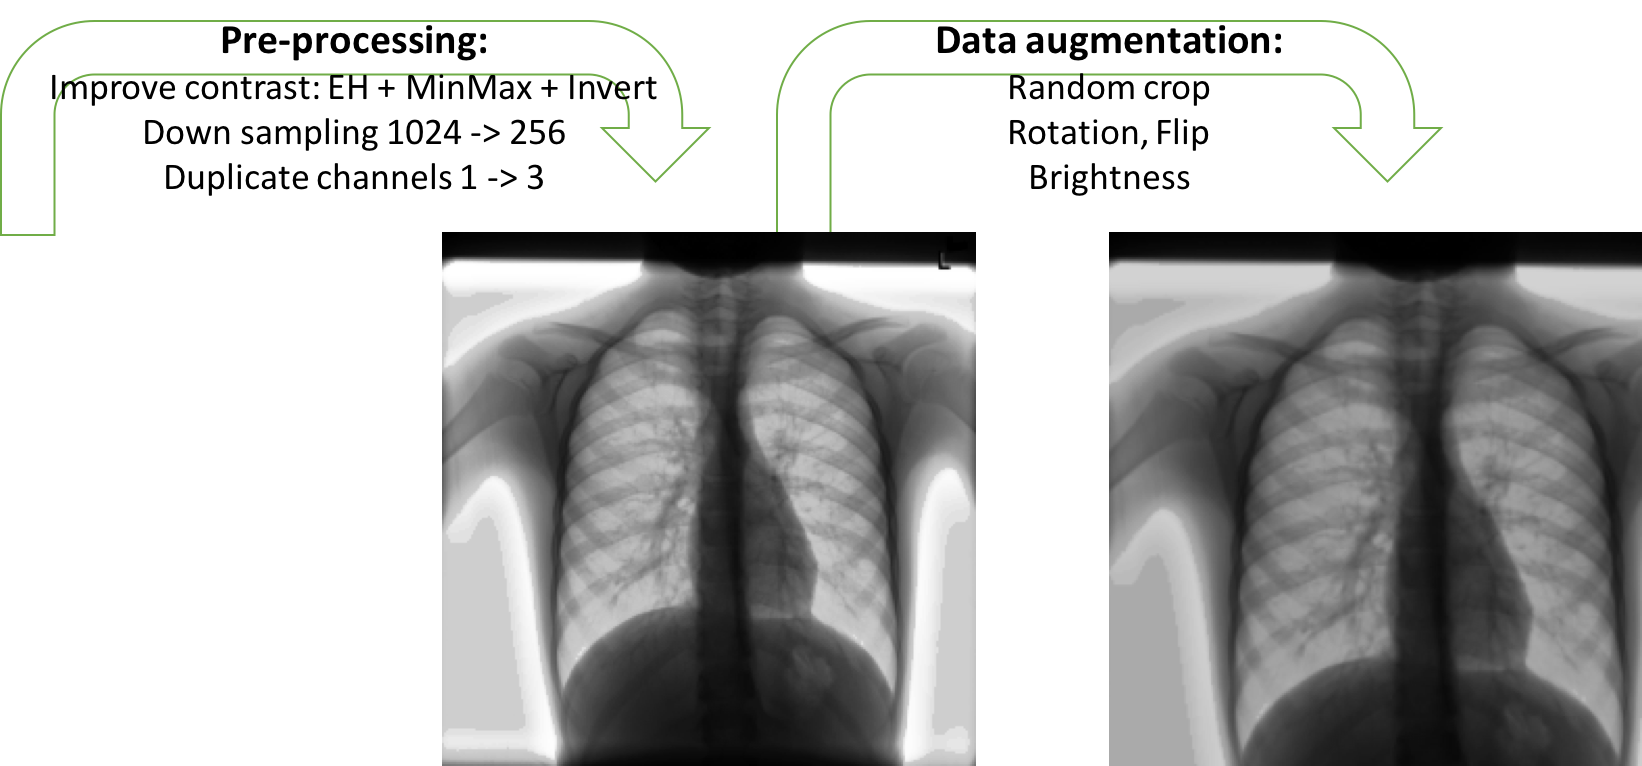
\includegraphics{dataAug_poster}

}
    \block{Models}{Content in your block.}
    \column{0.6}
    \block{Training}{Content in your block.}
    \block{Generalization Results}{Content in your block.}
    \block{Conclusion}{Content in your block.}
\end{columns}

\end{document}
